\documentclass{ieeeaccess}
\usepackage{cite}
\usepackage{amsmath,amssymb,amsfonts}
\usepackage{algorithmic}
\usepackage{graphicx}
\usepackage{textcomp}
\usepackage{booktabs}
\usepackage{multirow}
\usepackage{url}
\graphicspath{{figures/}}

\begin{document}

\history{Date of publication xxxx 00, 0000, date of current version xxxx 00, 0000.}
\doi{10.1109/TQE.2020.DOI}

\title{Calibration-Free Estimation of the Gate-Pair Atom-Loss Correlation in
Neutral-Atom Surface Codes}

\author{\uppercase{Suriya Narayanan Rajavel}\authorrefmark{1}}
\address[1]{Department of Applied Data Science, University of Florida, Gainesville, FL 32611 USA (email: suriyarajavel02@gmail.com)}

\markboth
{Rajavel: Calibration-Free Estimation of Gate-Pair Atom-Loss Correlation}
{Rajavel: Calibration-Free Estimation of Gate-Pair Atom-Loss Correlation}

\corresp{Corresponding author: Suriya Narayanan Rajavel (email: suriyarajavel02@gmail.com).}

\begin{abstract}
Atom loss is one of the main errors on neutral-atom processors. A Rydberg gate
that ejects one atom can eject its partner as well, and the conditional
probability of that second loss is a device parameter. Two recent studies sweep
it from $0$ to $1$ and find that published loss thresholds move by up to roughly fifty
percent. Both leave the number unspecified, since existing routes to measuring it need
loss-resolving readout or extra detection hardware. This paper recovers it
from the measurement record of an ordinary surface-code memory experiment.
When a gate loses a data atom, the partner ancilla's outcome is set by one of
two constants, fixed by the code and by empty-trap readout rather than by a
fit: one value if the partner survived, the other if it was lost as well. The
recorded dark rate mixes the two; inverting the mixture gives the correlation. No extra circuit, calibration experiment, or trained model is
required. We test the formula against known answers on three code families and
three distances, under a noise model that includes biased errors on surviving atoms and the measured
two-qubit gate error budget, and we report how the shot cost grows when the
preceding loss-localization step is imperfect.
\end{abstract}

\begin{keywords}
Atom loss, calibration, device characterization, erasure channel, neutral-atom
quantum computing, parameter estimation, quantum error correction, Rydberg atoms,
surface code, syndrome measurement.
\end{keywords}

\titlepgskip=-15pt
\maketitle


\section{Introduction}
\label{sec:introduction}

\PARstart{N}{eutral}-atom processors have become a leading platform for quantum
error correction~\cite{bluvstein2024logicalprocessor}, but they carry an error
that superconducting~\cite{acharya2023scalingsurfacecode,acharya2024belowthreshold}
and trapped-ion systems do not share at comparable rates: atoms are physically
lost from their traps. In a recent high-fidelity entangling-gate demonstration,
atom loss accounted for roughly half of the two-qubit error budget,
$0.061\%$ per gate against $0.035\%$ leakage, $0.024\%$ Pauli-$Z$, and
$0.003\%$ Pauli-$X(Y)$~\cite{evered2026highfidelitygates}. Loss is not a Pauli
error. A lost qubit leaves the computational space, so the stabilizers supported
on it become undefined rather than flipped, and decoders written for Pauli noise
do not describe the record without modification.

Rydberg gates add a second complication. The two atoms are brought into
interaction range, and the mechanisms that eject one of them---anti-trapping in
the Rydberg state, radiative decay to untrapped levels---can eject both. The
relevant quantity is
\begin{equation*}
  \eta = \Pr\!\left[\text{partner atom lost} \,\middle|\, \text{this atom lost in the same gate}\right],
\end{equation*}
the conditional probability that a gate which loses one atom loses both. The
same parameter appears as $p_c$ in Ref.~\cite{perrin2026correlatedloss} and
under the present symbol in Ref.~\cite{liu2026optimaldistanceatomloss}.

It has not been measured on a device. Both of those studies treat $\eta$ as a
free input and sweep it from $0$ to $1$, and the sweep is not cosmetic.
Ref.~\cite{perrin2026correlatedloss} finds the loss threshold moving from
$3.2\%$ to $4\%$ as the correlation increases;
Ref.~\cite{liu2026optimaldistanceatomloss} reports the corresponding threshold
moving from $5.15\%$ to $7.82\%$. Those are changes of twenty-five and roughly fifty percent in performance
predictions, attached to a parameter that neither paper can determine for a
particular array. Measuring it has so far required either loss-resolving
readout, available in metastable encodings through erasure
conversion~\cite{wu2022erasureconversion,ma2023midcircuiterasure}, or
teleportation-based loss-detection units inserted into the syndrome-extraction
circuit~\cite{perrin2026correlatedloss}. Neither is present in a standard
surface-code memory experiment.

Both studies also find that correlated loss raises the threshold rather than
lowering it, which can make the exact value look secondary. It is not, because
the reported benefit varies continuously with $\eta$. A device at $\eta=0.3$ and
a device at $\eta=0.9$ occupy different points on the published curves, with
different resource estimates and a different answer to whether
correlated-loss-aware decoding is worth implementing. Those papers quantify the
payoff as a function of the parameter; they do not determine which payoff a
given device receives.

We show that $\eta$ can be recovered in closed form from the raw measurement
record that a surface-code memory experiment already produces. The estimator
rests on two constants fixed by the code structure and the readout mechanism
rather than by a fit. When a data qubit is lost and its gate partner survives,
the truncated stabilizers anticommute and the partner ancilla's outcome is
unbiased. When the partner is co-lost, that ancilla is absent at readout and
cannot be bright, up to a false-bright rate that can be measured on an empty
trap. The observed rate is a mixture of the two cases, and inverting the mixture
gives $\eta$ directly.

This paper makes six contributions.

\begin{enumerate}
  \item A closed-form estimator for the gate-pair atom-loss correlation, built
        from two theory-pinned constants and one directly measurable hardware
        parameter. It does not require loss-resolving readout, loss-detection
        circuitry, a dedicated calibration experiment, or a trained model.
  \item Validation against known answers rather than against a second
        implementation of the same pipeline. The first constant is verified by
        forced injection over $9.6\times10^{6}$ samples and is uniform across
        data-qubit degree, ancilla type, and gate substep; the second is exact
        across $12\,473$ co-loss events. The remaining
        pipeline is gated behind a suite of thirty known-answer checks.
  \item A quantitative account of why the detector representation used in this
        literature cannot deliver the same estimate. The parity of consecutive
        rounds is what makes syndrome data informative for Pauli noise, and it
        is also what destroys the loss signature on any stabilizer whose sign
        was randomly projected. We state this as a prediction, measure the
        resulting gap, and confirm that it applies as well to the two-step
        construction developed for leakage
        detection~\cite{bultink2020repetitiveparity,varbanov2020leakagedetection}.
  \item Demonstration across three code families and three code distances, with
        the gate schedule detected from the circuit rather than assumed,
        including a color code whose layer count and stabilizer sign structure
        both differ from the surface code.
  \item Characterization of the shot cost as a function of the quality of the
        upstream loss-localization step. A localizer that is wrong three times
        in four costs a factor of roughly three in precision, so the method
        does not require a strong loss decoder.
  \item An explicit negative result. Supplying the estimated correlation to a
        decoder that discounts syndrome bits from co-lost ancillas does not
        reduce the logical error rate, for a reason internal to the estimator's
        own physics. We report this together with the control that establishes
        the null is real.
\end{enumerate}

Using raw stabilizer outcomes in place of detector differences is not a novel
input representation. It is established for leakage detection in superconducting
devices~\cite{bultink2020repetitiveparity,varbanov2020leakagedetection} and has
been applied to atom loss by a learned decoder that consumes raw outcomes and
detectors as separate features~\cite{wang2026aiqubitloss}. The contribution
here is the estimand and the closed form, together with the measured
representation gap and the argument that accounts for it.

The rest of the paper is organized as follows.
Section~\ref{sec:related} reviews atom loss in neutral-atom error correction,
prior treatments of correlated loss, existing work that reads loss from the
syndrome record, and the syndrome-statistics estimation literature.
Section~\ref{sec:theory} develops the loss model, the two anchors, the
estimator, the argument for detector blindness, two systematic corrections, and the measurement procedure as it would run on hardware.
Section~\ref{sec:methods} describes the simulation, the loss-injection
procedure, the known-answer checks, the baselines, and the refined noise model.
Section~\ref{sec:results} reports the results.
Section~\ref{sec:discussion} discusses scope and limitations, and
Section~\ref{sec:conclusion} concludes.


\section{Background and Related Work}
\label{sec:related}

\subsection{Atom Loss and Its Correction}
\label{sec:rel-loss}

Loss on a neutral-atom array has several sources~\cite{morgado2021rydbergreview}.
During a Rydberg gate the excited state is anti-trapped in a standard tweezer,
so an atom still in the Rydberg state at the end of the pulse can leave.
Radiative decay can land in levels the trap does not hold. Background-gas
collisions and imperfect recapture during imaging add loss off the gate.
Ref.~\cite{evered2026highfidelitygates} quotes $0.054\%$ loss per atom per gate
and splits the two-qubit error into $0.061\%$ loss, $0.035\%$ leakage,
$0.024\%$ Pauli-$Z$, and $0.003\%$ Pauli-$X(Y)$. Loss is the largest piece.

A Pauli error stays in the computational space and flips the anticommuting
stabilizers~\cite{terhal2015qecreview}. A matching decoder can use that flip.
A lost atom is gone. The stabilizers on it are undefined, and the corresponding
outcomes stay uninformative for the rest of the run instead of appearing as one
isolated flip.

The usual fix is to turn loss into erasure. If the missing qubit is known, the
error is a Pauli of known support and unknown type, which is easier than an
error of unknown location. Ref.~\cite{delfosse2020erasuredecoding} gives a
linear-time maximum-likelihood decoder for the surface code on the erasure
channel. Refs.~\cite{stace2009lossthresholds,stace2010degeneracyloss} merge
stabilizers that touched the lost qubit into superstabilizers on the survivors,
at the price of a lower effective distance. Later loss-tolerant decoders use
the same idea; Refs.~\cite{baranes2026lossdetection,baranes2025architecture}
write the superchecks in a fault-tolerant algorithmic setting.

All of that assumes known loss locations. Three ways to get them exist.
Erasure conversion puts the qubit in a metastable manifold so the dominant
error decays to a state that is not either computational level, and can be
caught mid-circuit~\cite{wu2022erasureconversion}. That has been shown in
Rydberg simulators~\cite{scholl2023erasurerydberg} and in gate
experiments~\cite{ma2023midcircuiterasure}. Loss-detection units insert a
teleportation circuit into the syndrome cycle and herald presence or
absence~\cite{perrin2026correlatedloss}. A decoder can also try to infer
locations from the syndrome record itself; that is
Sec.~\ref{sec:rel-syndrome}. The first two need hardware that a standard memory
experiment does not have. The third does not. That is the setting used here.
A related line finds Rydberg decay events inside leakage-reduction
circuits~\cite{yu2026rydbergdecayswaplrc}.

\subsection{Correlated Atom Loss}
\label{sec:rel-correlated}

A Rydberg gate acts on two atoms at once, so a loss at that gate need not be an
independent single-atom event. Ref.~\cite{perrin2025qecatomloss} noted the
possibility and set it aside: each gate gets a loss probability $p_l$, both
atoms are lost with probability $p_l^2$, and genuinely correlated loss is left
for later work.

That later work is Ref.~\cite{perrin2026correlatedloss}. It adds a second
parameter, the conditional probability of losing the second atom given that the
first was lost in the same gate. The decoder builds a loss graph from heralds
produced by teleportation-based detection units and updates per-edge loss
posteriors. Relative to a decoder that assumes independent loss, they report up
to an order-of-magnitude drop in logical error probability and a threshold
increase from $3.2\%$ to $4\%$. The correlation itself is an a priori input,
swept from $0$ to $1$.

Ref.~\cite{liu2026optimaldistanceatomloss} reaches a similar conclusion from a
different construction. The appendix parameterizes an error rate $p$ and a
correlated-loss weight $\eta$ so that each atom is lost alone with probability
$p(1-\eta)/2$ and both are lost together with probability $p\eta/2$. Correlated
loss then has the same effective distance as Pauli errors. The threshold rises
from $5.15\%$ to $7.82\%$ as $\eta$ goes from $0$ to $1$. Again $\eta$ is a
simulation input, and the decoders in that paper assume loss-resolving readout.

Nearby papers from the same line treat other parts of the loss channel.
Ref.~\cite{pecorari2026lossbiased} ionizes spurious Rydberg excitations
mid-circuit to push the noise toward a detectable channel, then argues that
loss-aware decoding approaches erasure scaling.
Ref.~\cite{jandura2026stabilizermeasurements} looks at how gate-level protocol
choices send leakage and decay into the stabilizer outcomes.

The pattern is consistent. The correlation is defined, swept, and shown to
matter. It is never read off data. Every quantitative claim about what it does
is conditional on a value that no published method can assign to a specific
device.

\subsection{Extracting Loss Information from the Syndrome Record}
\label{sec:rel-syndrome}

The raw stabilizer record holds information that the detector record drops.
That observation is older than this paper and first appeared for leakage, not
loss. Ref.~\cite{bultink2020repetitiveparity} finds leaked ancillas on a
superconducting device from the repeated parity record: a leaked ancilla
returns a fixed outcome because the measurement cannot tell the leaked state
from one computational level. They form a two-step syndrome from measurements
two rounds apart, because the usual consecutive-round detector erases that
signature. Ref.~\cite{varbanov2020leakagedetection} extends the same record to
a transmon surface code with hidden Markov models.

For atom loss, Ref.~\cite{wang2026aiqubitloss} decodes loss events from the
stabilizer record with no detection units and no special atomic species. The
physical handle is the same one used here. A lost data qubit makes overlapping
stabilizers anticommute, so the affected outcomes collapse to either sign with
equal probability. The result is temporally correlated flicker, not a single
flip. They feed a spatio-temporal graph network both the raw bit and the
detector value and report recall $0.654$ at precision $0.845$ over ten rounds
at distance five. That paper sits in a larger line of learned topological
decoders~\cite{torlai2017neuraldecoder,varsamopoulos2018feedforward,baireuther2018mlassisted,chamberland2018deepneuraldecoders,bausch2024alphaqubit}.

So raw outcomes versus detectors, for loss, is not original to this work.
Three things differ from Ref.~\cite{wang2026aiqubitloss}. The estimand is a
parameter of the loss model, not a list of loss locations. The method is
closed-form with constants fixed by the code, not a network whose accuracy
tracks its training distribution. The loss model here has a correlation
parameter; theirs is round-level independent loss, so $\eta$ does not appear.
The two jobs fit together. A localizer of the kind they train is a natural
front end for the estimator below; Sec.~\ref{sec:res-localizer} puts a number
on that pairing.

What this paper adds on representation is a measurement and an argument, not a
new data format. Prior work chose raw outcomes. It did not measure what that
choice is worth, and it did not say when the detector record has to fail. Both
are below. In particular, the two-step construction of
Refs.~\cite{bultink2020repetitiveparity,varbanov2020leakagedetection} does not
recover the atom-loss signature. The reason is the same one given in
Sec.~\ref{sec:theory-detector}.

\subsection{Estimating Error-Model Parameters from Syndrome Data}
\label{sec:rel-estimation}

Reading error rates out of syndrome data is a separate, mature line.
Ref.~\cite{spitz2018adaptiveweight} introduced the pairwise estimator that
recovers effective error probabilities from correlations between detector
events, so matching weights can follow measured noise.
Ref.~\cite{blumekohout2025detectorerrormodels} puts that on a general footing:
probabilities of individual and aggregated detector-error-model events, from
multi-cycle data, with the pairwise estimator as a special case. A parallel
line estimates Pauli channels on the extraction circuit;
Ref.~\cite{hockings2025aces} estimates circuit eigenvalues from raw
measurements at scale.

Two facts about that literature matter here. First, the target is Pauli and
measurement error. For those mechanisms the detector record is the right
object: the information lives in changes of stabilizer value, and the
detector map isolates those changes while dropping a gauge that carries
nothing. Second, the whole program therefore starts from detector histories.
Both Ref.~\cite{spitz2018adaptiveweight} and
Ref.~\cite{blumekohout2025detectorerrormodels} take the parity of consecutive
rounds before they estimate anything.

That parity step is where atom loss disappears. A lost atom pins an outcome
to a fixed value, gauge or no gauge, so the map that removes the gauge also
removes the signature on any stabilizer whose sign was randomly projected
(Sec.~\ref{sec:theory-detector}). Sec.~\ref{sec:res-representation} measures
the gap. Those estimators are not rivals on the same task. Their input
representation does not contain the error class treated here.

\subsection{Position of This Work}
\label{sec:rel-position}

Table~\ref{tab:priorwork} asks two questions of each related method: does it
treat the correlation at all, and if it does, does it read the number from
data or take it as an input?

\begin{table}[!t]
\caption{Treatment of the gate-pair loss correlation in related work.
``Swept'' means the parameter is a simulation input. ``Estimated'' means it
is inferred from measured data.}
\label{tab:priorwork}
\centering
\begin{tabular}{@{}llll@{}}
\toprule
Work & Correlation & Source & Extra hardware \\
\midrule
\cite{spitz2018adaptiveweight,blumekohout2025detectorerrormodels} & not modeled & --- & none \\
\cite{hockings2025aces} & not modeled & --- & none \\
\cite{wang2026aiqubitloss} & not modeled & --- & none \\
\cite{perrin2025qecatomloss} & independent & assumed & LDUs \\
\cite{perrin2026correlatedloss} & modeled & swept & LDUs \\
\cite{liu2026optimaldistanceatomloss} & modeled & swept & loss readout \\
\cite{pecorari2026lossbiased} & modeled & swept & ionization \\
\midrule
This work & modeled & \textbf{estimated} & \textbf{none} \\
\bottomrule
\end{tabular}
\end{table}

Methods that need no extra hardware do not model the correlation. Either they
target a different error class
\cite{spitz2018adaptiveweight,blumekohout2025detectorerrormodels,hockings2025aces}
or their loss model has no $\eta$ \cite{wang2026aiqubitloss}. Methods that do
model the correlation take it as an input and also assume loss-resolving
readout or detection circuitry
\cite{perrin2026correlatedloss,liu2026optimaldistanceatomloss,pecorari2026lossbiased}.
No published method estimates the parameter from an unmodified
syndrome-extraction experiment.

That is the setting of this paper. We do not claim a better decoder than
Refs.~\cite{perrin2026correlatedloss,liu2026optimaldistanceatomloss}: those
constructions solve a different problem and rely on hardware we do not assume.
What they need, and do not currently measure, is the value of $\eta$. We also
do not claim a better estimator of Pauli or measurement rates than
Refs.~\cite{spitz2018adaptiveweight,blumekohout2025detectorerrormodels}; those
methods are correctly built on the detector record. Finally, we do not claim
to have introduced raw-outcome loss inference, which
Refs.~\cite{bultink2020repetitiveparity,varbanov2020leakagedetection,wang2026aiqubitloss}
already use. The point of the derivation below is to show what that record
makes available in closed form, and to measure what is lost if one uses
detectors instead.


\section{Estimating the Loss Correlation from Syndrome Measurements}
\label{sec:theory}

\subsection{Loss Model and the Correlation Parameter}
\label{sec:theory-model}

Loss is modeled at individual two-qubit gates. Following the parameterization
already used in this
literature~\cite{perrin2026correlatedloss,liu2026optimaldistanceatomloss},
\begin{equation}
  \eta \;=\; \Pr\!\left[\text{partner atom lost} \,\middle|\, \text{this atom lost in the same CZ}\right],
  \label{eq:eta-def}
\end{equation}
is the chance that a gate which loses one atom loses both. For a gate on atoms
$(a,b)$ with per-atom loss probability $p_g$,
\begin{align}
  \Pr[\text{both lost}] &= \eta\,p_g, \label{eq:both}\\
  \Pr[\text{only } a] = \Pr[\text{only } b] &= (1-\eta)\,p_g. \label{eq:one}
\end{align}
The per-atom marginal is $p_g$ for any $\eta$. That matching matters. If
varying $\eta$ also changed the total loss budget, no observable could be
blamed on correlation alone.

Equations~\eqref{eq:both}--\eqref{eq:one} match
Ref.~\cite{liu2026optimaldistanceatomloss} under $p=2p_g$: each atom is lost
alone with probability $p(1-\eta)/2$ and together with its partner with
probability $p\eta/2$. They also match $p_c$ in
Ref.~\cite{perrin2026correlatedloss}.

In a surface-code extraction circuit every two-qubit gate is data--ancilla.
There are no data--data entangling gates. The partner of a lost data qubit,
when the loss is correlated, is always an ancilla. Ancillas are reset and
measured every round, so ancilla loss is transient. Data loss lasts for the
rest of the experiment. The estimator uses that asymmetry.

\subsection{Two Theory-Pinned Anchors}
\begin{figure}[!t]
\centering
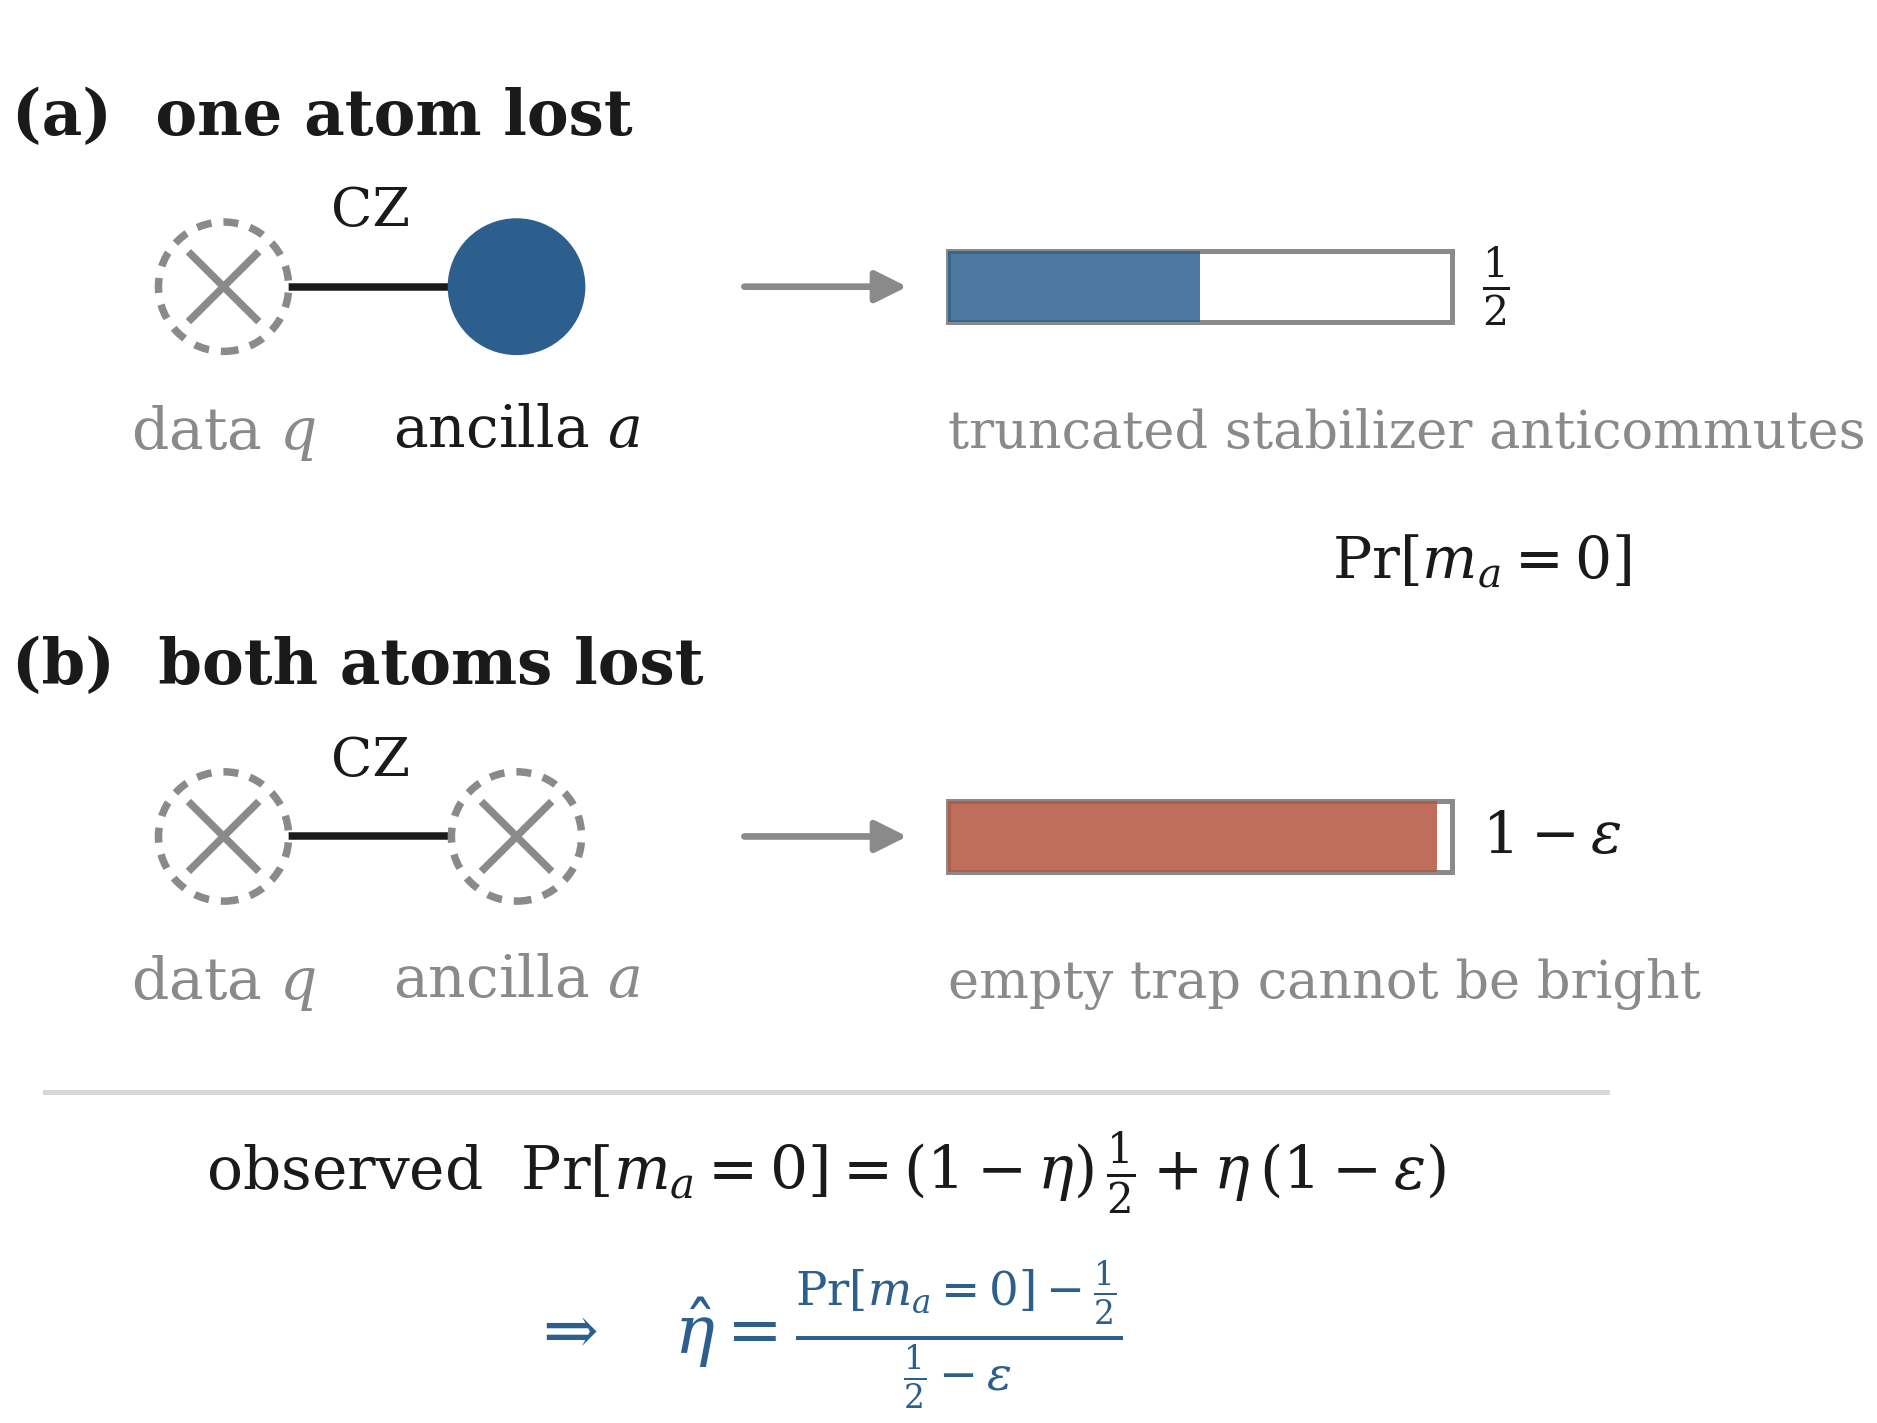
\includegraphics[width=\columnwidth]{figures/fig1_mechanism.png}
\caption{How the estimator works. A two-qubit gate couples a data qubit to an
ancilla. (a)~Only the data qubit is lost: the stabilizers on it are truncated
and anticommute, so the surviving partner ancilla is unbiased. (b)~Both atoms
are lost: the ancilla is missing at readout and cannot be bright, up to the
false-bright rate $\epsilon$. The recorded rate is a mixture weighted by
$\eta$. Inverting the mixture recovers $\eta$. Neither constant is fitted.}
\label{fig:mechanism}
\end{figure}
\label{sec:theory-anchors}

Take a data qubit lost during a gate, and let $a$ be the ancilla on that gate.
Let $m_a$ be the raw outcome of that ancilla in the loss round.
Fig.~\ref{fig:mechanism} is the two-case picture.

If the partner ancilla survives, the lost data qubit truncates the stabilizers
that used it. The truncated $X$-type and $Z$-type operators anticommute, so
the measured bit is $\pm 1$ with equal probability:
\begin{equation}
  \Pr[m_a = 0 \mid \text{partner alive}] = \tfrac{1}{2}.
  \label{eq:anchor1}
\end{equation}

If the partner is lost as well, it is absent at readout and cannot be bright.
Array readout looks for population in the excited state, so an empty trap looks
like the ground state, except for a false-bright rate $\epsilon$ from dark
counts or stray scatter:
\begin{equation}
  \Pr[m_a = 0 \mid \text{partner co-lost}] = 1-\epsilon.
  \label{eq:anchor2}
\end{equation}

Neither number is fitted. Equation~\eqref{eq:anchor1} is the code.
Equation~\eqref{eq:anchor2} is the readout. $\epsilon$ is measured on an empty
trap.

\subsection{The Estimator}
\label{sec:theory-estimator}

A fraction $\eta$ of loss events are co-loss events, so the observed dark rate
mixes \eqref{eq:anchor1} and \eqref{eq:anchor2}. Invert the mixture:
\begin{equation}
  \hat\eta \;=\; \frac{\Pr[m_a=0] - \tfrac{1}{2}}{\tfrac{1}{2}-\epsilon}.
  \label{eq:estimator}
\end{equation}
A binomial interval on $\Pr[m_a=0]$ maps through the same linear function.
Equation~\eqref{eq:estimator} has no fitted parameters. It does not need a
loss-detection unit, loss-resolving readout, or a calibration experiment. It
does need loss events localized well enough to know which ancilla to read.
Sec.~\ref{sec:res-localizer} puts a number on that requirement.

\subsection{Why the Detector Representation Is Blind to Loss}
\label{sec:theory-detector}

Decoders and most syndrome-statistics estimators do not see raw outcomes.
They see detectors, the parity of consecutive rounds,
\begin{equation}
  d_a(r) = m_a(r) \oplus m_a(r-1).
  \label{eq:detector}
\end{equation}
For Pauli noise that is the right map. The absolute stabilizer value after
the first round is a random projection and carries no information; only later
changes matter.

The same map removes the loss signature. A dead ancilla gives $m_a(r)=0$
every time, so $d_a(r)=m_a(r-1)$, last round's raw bit. Two cases follow.
If the stabilizer sign is deterministic in the memory basis, then
$m_a(r-1)=0$ and the detector is $0$, which is not the $1/2$ expected from a
surviving truncated ancilla. If the sign was a random projection, then
$m_a(r-1)$ is an unbiased bit and the detector is a coin flip, identical to a
surviving truncated ancilla.

Half the ancillas in a surface-code memory experiment measure randomly
projected stabilizers. On that half the detector record does not say whether
the partner was co-lost. The raw outcome is $0$ in both cases, and that is
usable. The prediction is therefore: co-loss discrimination is essentially
complete in the raw record for both ancilla types; strong in the detector
record for the deterministic type; absent in the detector record for the
projected type. Sec.~\ref{sec:res-representation} tests that split, including
against the two-step object $s_a(r)=m_a(r)\oplus m_a(r-2)$ used for leakage
detection~\cite{bultink2020repetitiveparity,varbanov2020leakagedetection}.
That construction differences against a round that is itself randomly
projected, so it is predicted to be blind as well.

The argument cares only about whether the sign was randomly projected, not
about which code produced the sign. Which ancilla type is blind depends on
basis and code. That the projected type is blind does not.

\subsection{Systematic Corrections}
\label{sec:theory-rules}

Equation~\eqref{eq:anchor1} is a steady-state statement. Two situations
violate it.

At the start of the experiment the data register is a product state. A
truncated memory-basis stabilizer is then still deterministic and reads $0$
with high probability. First-round losses are dropped.

Data loss is permanent, so a stabilizer truncated in round $r$ stays
truncated. After the first truncated outcome, the surviving qubits are
projected and later rounds are deterministic. Only the first truncated round
obeys \eqref{eq:anchor1}. Restricting to first-truncation events removes that
bias. Sec.~\ref{sec:res-estimator} shows that, at physical loss rates, dropping
the first round is already enough. The persistence cut only starts to matter
well above hardware $p_g$.

\subsection{Procedure on a Memory Experiment}
\label{sec:theory-protocol}

What follows is the measurement one would run on hardware. It is not a
hardware result; every number in this paper is still from simulation. The
point is that the inputs already sit in a standard memory run.

Measure $\epsilon$ once, on traps known to be empty, with the same imaging
settings used in the experiment. That is the only extra shot budget, and it
is small. Then run the usual surface-code memory experiment and keep the raw
ancilla outcomes. Detectors can still be built for decoding; the estimator
does not use them.

For each candidate loss reported by the localizer, note the data qubit and the round, drop the
event if it falls in the first round, and keep only the first truncated
round on that qubit. Read the partner ancilla from that gate. If the
localizer does not return the gate substep, average the candidate partners
as in Sec.~\ref{sec:res-localizer}. The estimate is then
\eqref{eq:estimator} applied to the empirical dark rate of those bits, with
a binomial interval mapped through the same linear function.

In short: empty-trap $\epsilon$; raw bits, not detectors; drop round one; first truncation
only; invert the mixture. A localizer of published quality is enough for
$\sigma_\eta \approx 0.01$ at $10^{6}$ memory shots.


\section{Simulation Methods}
\label{sec:methods}

\subsection{Circuits and Noise}
\label{sec:methods-circuit}

All circuits are rotated surface-code memory experiments generated by
Stim~\cite{gidney2021stim}. Layout, extraction schedule, and detector
definitions come from Stim, not from a hand-built netlist, so the
hook-error-avoiding gate order is the usual
one~\cite{tomita2014lowdistancesurfacecodes}. Unless a caption says otherwise,
the setup is distance $d=5$, $T=12$ rounds, and uniform circuit-level
depolarizing noise at $p=2\times10^{-3}$ after Clifford gates, on data qubits
before each round, before measurement, and after reset. At $d=5$ that is $25$
data qubits and $24$ ancillas ($12$ of each type), with $80$ two-qubit gates
per round in four substeps of $20$. Each qubit takes part in at most one gate
per substep. All $80$ gates are data--ancilla and cover $80$ distinct Tanner
edges; there are no exceptions in the generated circuits.

Unless stated otherwise, $p_g=5.4\times10^{-4}$, the per-atom per-gate loss
probability in Ref.~\cite{evered2026highfidelitygates}. The marginal matching
in \eqref{eq:both}--\eqref{eq:one} was checked numerically at an elevated test rate of $p_g=10^{-2}$. At
$\eta=0.00,\,0.25,\,0.50,\,1.00$ the measured per-atom loss rate is
$0.00995,\,0.00998,\,0.01004,\,0.00992$ against a target of $0.01$, and the
co-lost fraction tracks $\eta$.

We also implemented the round-level independent loss model of
Ref.~\cite{wang2026aiqubitloss}, in which each qubit is removed with a fixed
probability each round. That is a different mechanism, not the $\eta\to 0$
limit of \eqref{eq:both}--\eqref{eq:one}. It is used only as an external
reference point. All quoted uncertainties in this paper are $95\%$ confidence intervals.

\subsection{Loss Injection}
\label{sec:methods-injection}

Atom loss is not a Pauli channel and is not injected as one. At the loss
instant we apply a single-qubit depolarizing channel of strength $3/4$. That
twirl is the completely depolarizing channel, so the atom is traced out and
replaced by the maximally mixed state. Every later operation on that qubit is
then stripped: a lost atom does not apply an entangling gate to a surviving
partner. The lost qubit's readout is forced to $0$ by a reset immediately
before the measurement, in the measurement basis. Ancillas come back on their
own mid-circuit reset each round; data qubits do not. Measurements are never
deleted, so the record length stays fixed and detector offsets stay valid.

Deleting a measurement would shift every later offset and silently break
downstream detectors. An invariant requires that measurement and detector
counts be independent of the loss configuration, in both memory bases.

\subsection{Known-Answer Validation}
\label{sec:methods-checks}

The statements in Sec.~\ref{sec:theory} have known answers, so the simulation
can be checked against those answers rather than against itself. A suite of
$30$ checks has to pass before any result is reported. The suite includes:
the noiseless circuit producing zero detector events; a no-loss rebuild that
matches the generated circuit exactly; the data--ancilla structure of every
two-qubit gate; a lost data qubit flickering exactly its Tanner-partner
ancillas and nothing else; $\eta$-independence of the loss marginals;
invariance of measurement and detector counts under loss in both bases;
byte-level agreement between an audited reference circuit builder and the
faster production builder, over $200$ random loss configurations in each
basis; both anchors of Sec.~\ref{sec:theory-anchors} at $\epsilon=0$ and
$\epsilon=0.02$; recovery of planted detector correlations by the baseline in
Sec.~\ref{sec:methods-baselines}; and the generality checks of
Sec.~\ref{sec:res-generality}.

Where a deterministic answer exists, injection is forced rather than sampled.
An earlier sampled version of the anchor check mixed in anomalous first-round
events and sat on the edge of its tolerance. Near the noise floor the checks
assert ratios, not absolute windows; a check that passes only some of the time
is not a check. The suite was rerun on two platforms and two Python versions.

\subsection{Baselines}
\label{sec:methods-baselines}

The comparison is to the detector-record estimators used in this
literature~\cite{spitz2018adaptiveweight,blumekohout2025detectorerrormodels}.
The pairwise estimator is implemented in the form given by Blume-Kohout and
Young~\cite{blumekohout2025detectorerrormodels},
\begin{equation}
  p_{ij} = \frac{1}{2} - \frac{1}{2}\sqrt{\frac{\langle z_i\rangle\langle z_j\rangle}{\langle z_i z_j\rangle}},
  \qquad z_i = (-1)^{d_i},
  \label{eq:pij}
\end{equation}
and checked on planted correlations ($p_{12}=0.05, 0.12, 0.03$ recovered as
$0.0504$, $0.1197$, $0.0300$; $0$ recovered as $-0.0005$). The two-step
syndrome of
Refs.~\cite{bultink2020repetitiveparity,varbanov2020leakagedetection} is
implemented as well. All three representations are scored on the same co-loss
discrimination task, split by ancilla type.

\subsection{Refined Neutral-Atom Physics}
\label{sec:methods-realism}

To move past a bare gate-cancellation loss model we add two effects reported
for these devices. Following Ref.~\cite{perrin2025qecatomloss}, when exactly
one atom of a gate pair is lost the surviving partner gets a maximally biased
$Z$ error, applied with probability $1/2$. The residual Pauli pieces of the
measured gate error budget in Ref.~\cite{evered2026highfidelitygates},
$0.024\%$ Pauli-$Z$ and $0.003\%$ Pauli-$X(Y)$, are applied to every surviving
gate. Loss and leakage are already carried by the loss channel. The
false-bright rate $\epsilon$ is swept from $0$ to $0.05$.

\subsection{Code-General Parsing}
\label{sec:methods-generality}

The rotated surface code has four gate layers per round; other codes do not.
The estimator does not assume the layer count. It parses the two-qubit layers,
finds the repetition period, and splits each layer into data--ancilla pairs.
The only requirements, checked per code, are that each qubit take part in at
most one gate per layer and that every gate be data--ancilla. Results are
reported for the rotated surface code at $d=3,5,7$; the unrotated surface
code~\cite{dennis2002topologicalmemory,fowler2012surfacecodes} at $d=5$, which
has a different stabilizer geometry but still four layers; and the color
code~\cite{bombin2006colorcodes} at $d=5$, a different family with six layers
per round.


\section{Results}
\label{sec:results}

\subsection{The Correlation Is Weakly Informative for Loss Detection}
\label{sec:res-ceiling}

Table~\ref{tab:ceiling} is a Bayes-optimal discrimination between a lost data
qubit and a surviving one: a likelihood-ratio test on the exact empirical
distribution of detector patterns on the victim's Tanner-partner ancillas. No
architecture looking at the same window can beat these numbers.

Going from $\eta=0$ to $\eta=1$ changes the AUC by at most $0.034$. The sign
of the change depends on the measurement basis and on whether the final destructive readout sits in the
window. After a lost qubit has had two rounds to flicker, the difference is
gone. Correlation is a poor prior for localizing loss.

Discriminating $\eta=1$ data from $\eta=0$ data, rather than lost qubits from
live ones, gives an AUC between $0.57$ and $0.75$, depending on basis and window.
That is the contrast the estimator uses.

\begin{table}[!t]
\caption{Bayes-optimal AUC for detecting a lost data qubit under uncorrelated
and fully correlated loss. $\Delta$ is the change from knowing the
correlation. The last row is the AUC that separates $\eta=1$ data from
$\eta=0$ data.}
\label{tab:ceiling}
\centering
\begin{tabular}{@{}llccc@{}}
\toprule
Window & Basis & $\eta=0$ & $\eta=1$ & $\Delta$ \\
\midrule
Final round, no final readout & $Z$ & 0.8426 & 0.8098 & $-0.033$ \\
Final round, with final readout & $Z$ & 0.8534 & 0.8874 & $+0.034$ \\
Final round, with final readout & $X$ & 0.9194 & 0.9120 & $-0.007$ \\
Early loss, two rounds flicker & $Z$ & 0.9871 & 0.9871 & $+0.000$ \\
Early loss, two rounds flicker & $X$ & 0.9873 & 0.9884 & $+0.001$ \\
\midrule
\multicolumn{5}{@{}l}{AUC discriminating $\eta=1$ from $\eta=0$ data: $0.57$--$0.75$} \\
\bottomrule
\end{tabular}
\end{table}

\subsection{Representation Dependence of the Co-Loss Signal}
\label{sec:res-representation}

Section~\ref{sec:theory-detector} says the detector map destroys the co-loss
signature on randomly projected stabilizers and that the raw record keeps it
everywhere. Table~\ref{tab:representation} is that test. The same partner
ancilla on the same events is scored three ways: the raw bit $m_a(r)$, the
one-step detector $m_a(r)\oplus m_a(r-1)$ used by matching decoders and by
Refs.~\cite{spitz2018adaptiveweight,blumekohout2025detectorerrormodels}, and
the two-step syndrome $m_a(r)\oplus m_a(r-2)$ of
Refs.~\cite{bultink2020repetitiveparity,varbanov2020leakagedetection}.

On the deterministic-sign ancilla type, all three representations work. On the
projected type the raw record still has a gap of $0.49$; both parity maps fall
to $0.003$ and $0.008$, consistent with zero. The two-step construction,
built for this kind of problem on superconducting devices, is blind here
because it differences against a randomly projected round
(Sec.~\ref{sec:theory-detector}).

\begin{table}[!t]
\caption{Co-loss discrimination gap on the partner ancilla, by representation
and ancilla type, memory-$Z$ experiment. The gap is
$|\Pr[\text{indicator}\,|\,\text{co-lost}] -
\Pr[\text{indicator}\,|\,\text{alive}]|$.}
\label{tab:representation}
\centering
\begin{tabular}{@{}lcc@{}}
\toprule
Representation & Deterministic & Projected \\
\midrule
Raw $m_a(r)$ & 0.501 & \textbf{0.486} \\
One-step $m_a(r)\oplus m_a(r-1)$ & 0.377 & \textbf{0.003} \\
Two-step $m_a(r)\oplus m_a(r-2)$ & 0.391 & \textbf{0.008} \\
\bottomrule
\end{tabular}
\end{table}

The pattern flips with the memory basis, as it should. In a memory-$Z$
detector record the deterministic $Z$-type ancillas carry a co-loss signal of
$+0.367$ and the $X$-type carry $-0.010$. In memory $X$ the numbers exchange:
$-0.001$ and $+0.374$. Blindness tracks the random projection, not the Pauli
label on the ancilla.

\subsection{Verification of the Anchors}
\label{sec:res-anchors}

Both constants in \eqref{eq:estimator} are fixed by theory, so they can be
tested rather than fitted. A single loss is injected at a bulk round and the
partner ancilla is read over $9.6\times10^{6}$ samples.

The first anchor holds to five digits:
$\Pr[m_a=0\,|\,\text{partner alive}]=0.49998\pm 0.00032$, a $-0.1\sigma$
deviation. Table~\ref{tab:anchors} splits the same data every way we could
think of. The value does not move, so it is not an average over a structured
population. The second anchor is exact at $\epsilon=0$: in $12\,473$ co-loss
events the partner's raw outcome was never $1$.

\begin{table}[!t]
\caption{First anchor, $\Pr[m_a=0\,|\,\text{partner alive}]$, by stratum.
Forced injection at a bulk round, $9.6\times10^{6}$ samples. Theory value
$0.5$.}
\label{tab:anchors}
\centering
\begin{tabular}{@{}llc@{}}
\toprule
Stratification & Stratum & $\Pr[m_a=0]$ \\
\midrule
\multirow{3}{*}{Data-qubit degree} & 4 (bulk) & $0.50006 \pm 0.00047$ \\
 & 3 (edge) & $0.49987 \pm 0.00047$ \\
 & 2 (corner) & $0.50017 \pm 0.00100$ \\
\midrule
\multirow{2}{*}{Ancilla type} & $Z$ & 0.49989 \\
 & $X$ & 0.50007 \\
\midrule
\multirow{4}{*}{Gate substep} & 0 & 0.50009 \\
 & 1 & 0.50001 \\
 & 2 & 0.49969 \\
 & 3 & 0.50014 \\
\midrule
\multicolumn{2}{@{}l}{Pooled} & $0.49998 \pm 0.00032$ \\
\bottomrule
\end{tabular}
\end{table}

\subsection{Recovery of $\eta$}
\begin{figure}[!t]
\centering
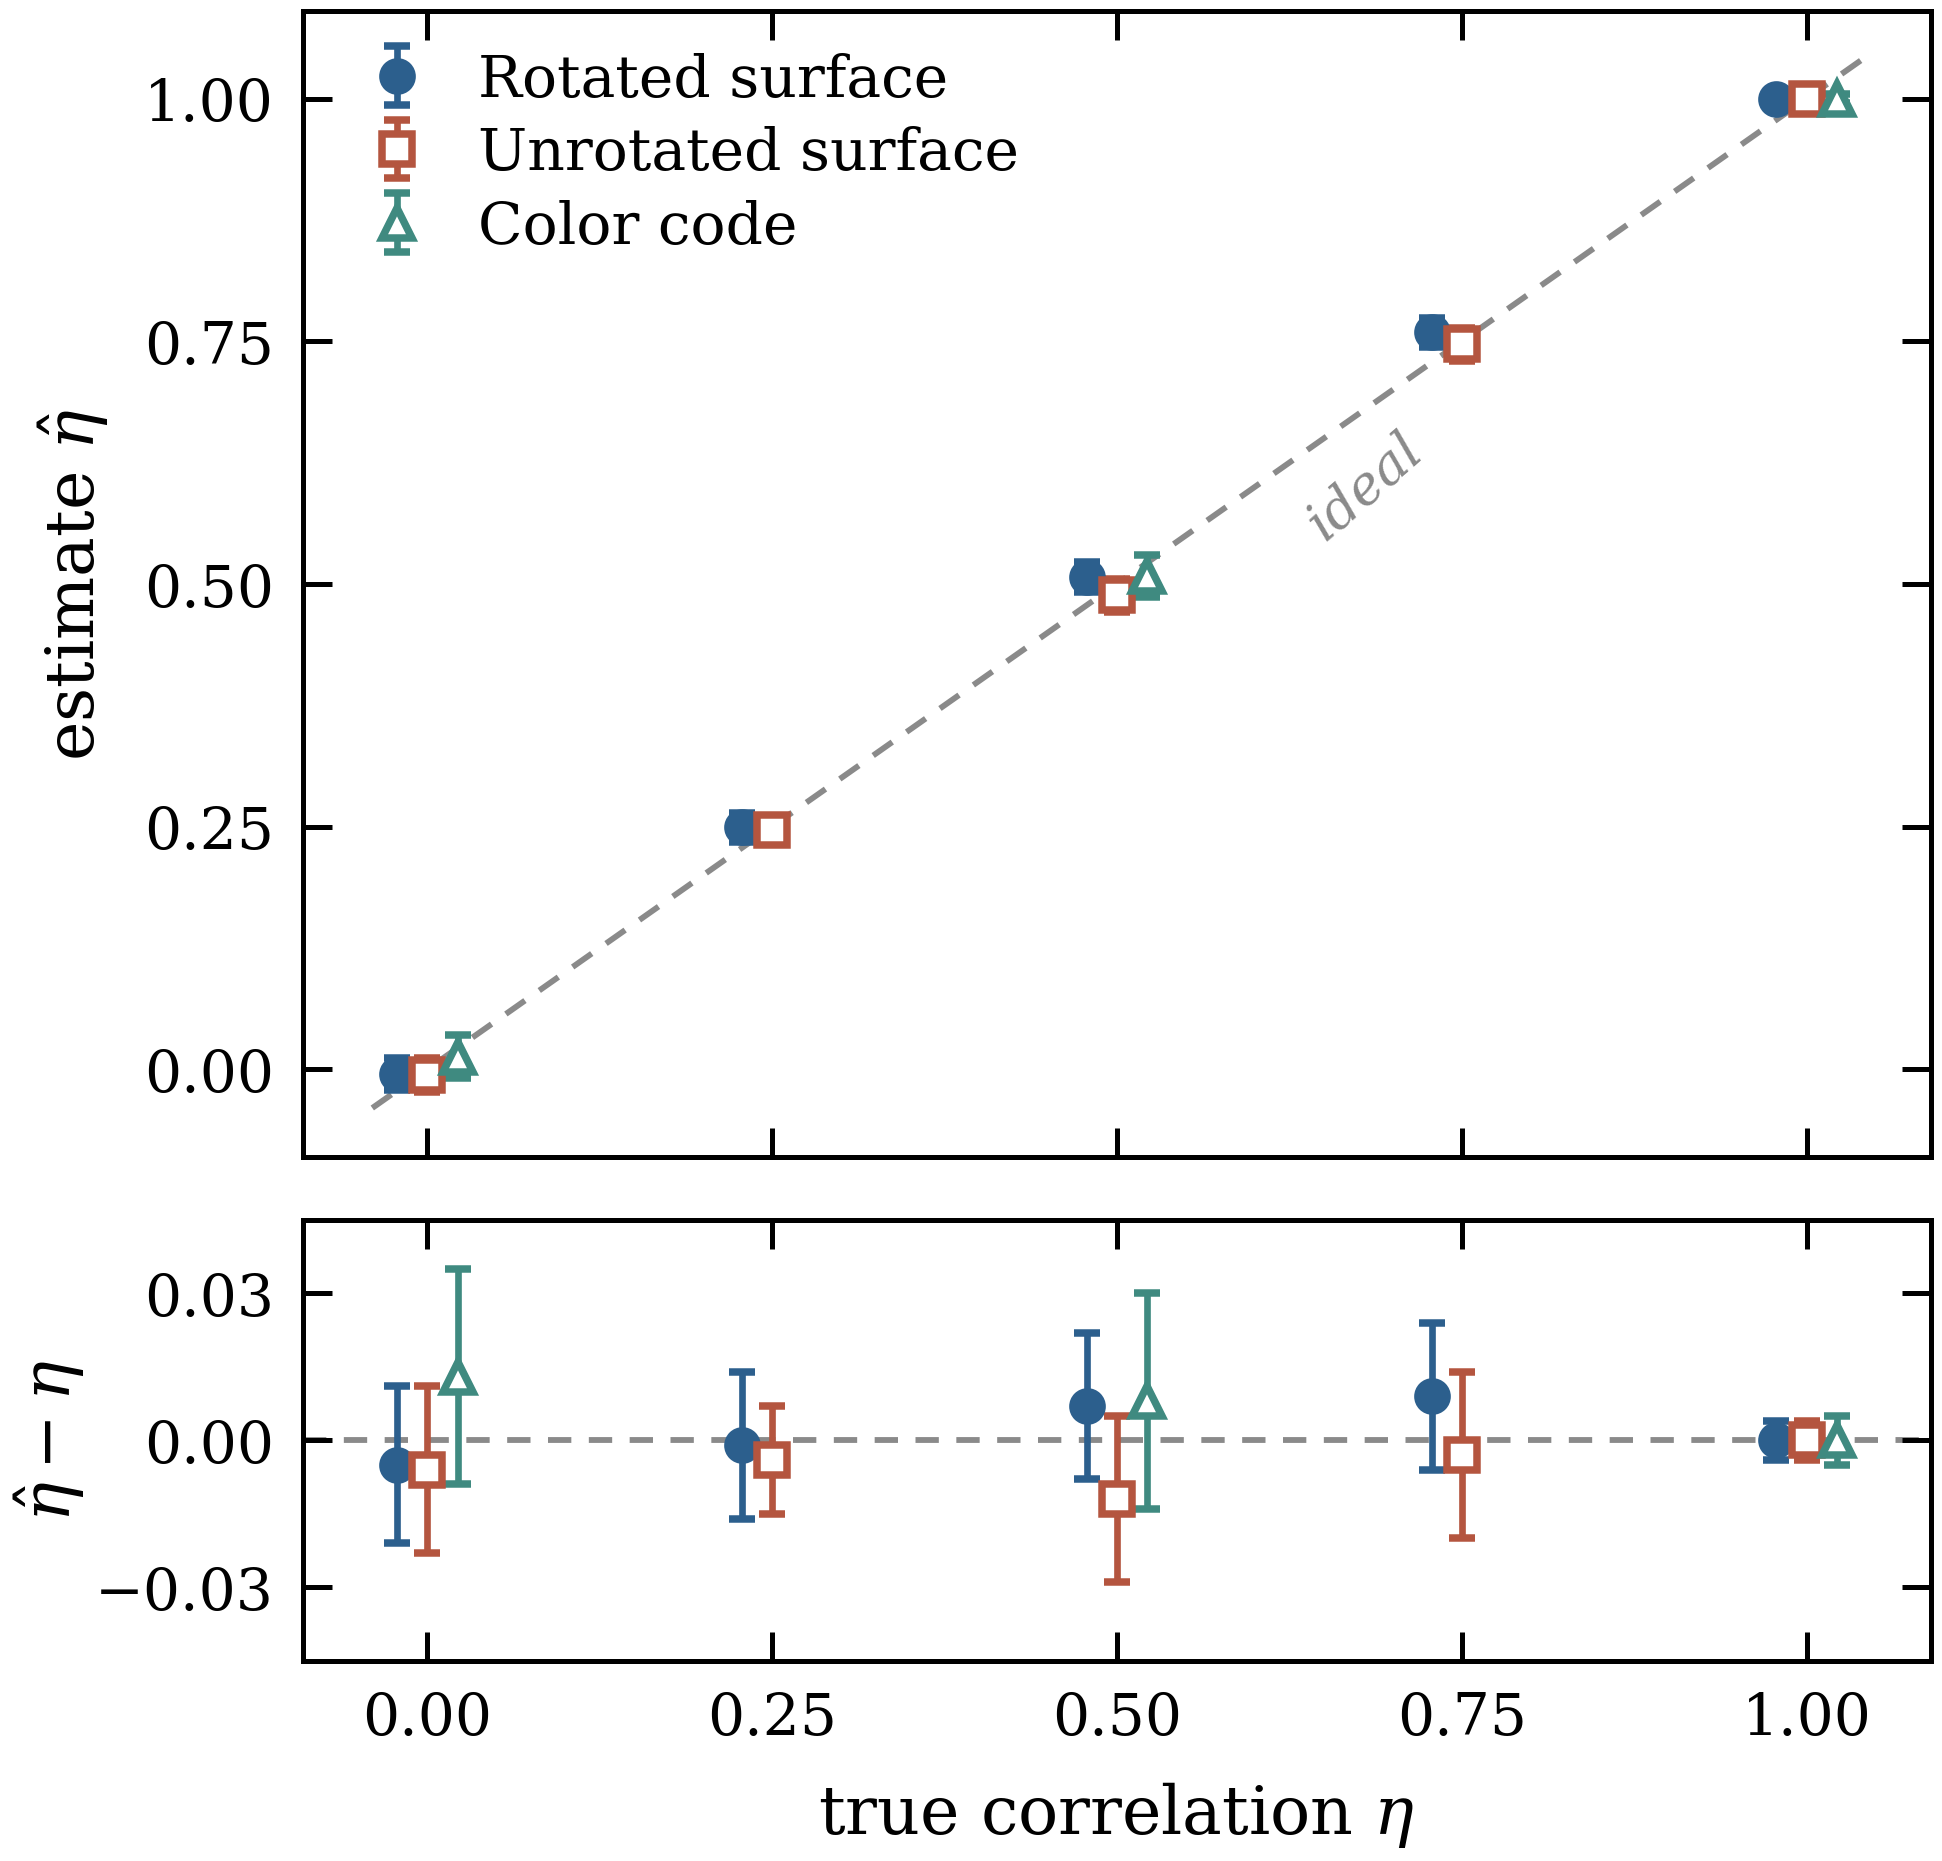
\includegraphics[width=\columnwidth]{figures/fig2_recovery.png}
\caption{Recovery of the gate-pair loss correlation across three code families
at $p_g=5.4\times10^{-4}$. Error bars are $95\%$ confidence intervals.
The color code has six two-qubit layers per
round rather than four, and a different stabilizer sign structure. Both were
read from the circuit, not assumed.}
\label{fig:recovery}
\end{figure}
\label{sec:res-estimator}

With the anchors in hand, \eqref{eq:estimator} is run on sampled correlated
loss at the physical rate $p_g=5.4\times10^{-4}$. For
$\eta_{\text{true}}=0.00$, $0.25$, $0.50$, $0.75$, $1.00$ the estimator
returns $-0.005$, $0.249$, $0.507$, $0.759$, $1.000$. Every point sits inside
its $95\%$ interval. Fig.~\ref{fig:recovery} shows the recovery. An independent seed gives $-0.006$, $0.255$, $0.510$, $0.751$, and $1.000$;
every point recovers its planted value inside its confidence interval, and the
two series agree to within $0.008$ at every $\eta$.

The two corrections in Sec.~\ref{sec:theory-rules} behave as written.
First-round losses give $\Pr[m_a=0]=0.6684\pm 0.0007$ for memory-basis
partners, against $0.5000$ in every later round, because the data register is
still a product state. With $T=12$ that predicts an upward bias of $+0.007$.
The pooled bias before correction is $+0.008$.

The persistence correction is visible only well above hardware $p_g$.
Table~\ref{tab:pgsweep} sweeps $p_g$ at $\eta_{\text{true}}=0$, so any nonzero
estimate is bias. At the physical rate the uncorrected estimator is already
unbiased. The extra cut becomes necessary only around ten times that rate.
Conditioning on ground truth at $p_g=10^{-2}$ shows the mechanism: events with
exactly one newly lost neighbor, which a naive collector treats as clean, read
$0.5242\pm 0.0049$, a $9.6\sigma$ shift from stabilizers truncated in an
earlier round that have since gone deterministic.

\begin{table}[!t]
\caption{Estimator bias at $\eta_{\text{true}}=0$ versus per-atom loss rate,
with and without the first-truncation restriction. The physical rate is
$5.4\times10^{-4}$.}
\label{tab:pgsweep}
\centering
\begin{tabular}{@{}lcc@{}}
\toprule
$p_g$ & Uncorrected & First-truncation only \\
\midrule
$5.4\times10^{-4}$ & $-0.0118 \pm 0.0164$ & $\phantom{-}0.0085 \pm 0.0169$ \\
$2\times10^{-3}$ & $\phantom{-}0.0083 \pm 0.0125$ & $\phantom{-}0.0107 \pm 0.0136$ \\
$5\times10^{-3}$ & $\phantom{-}0.0353 \pm 0.0112$ & $-0.0047 \pm 0.0136$ \\
$1\times10^{-2}$ & $\phantom{-}0.0590 \pm 0.0098$ & $\phantom{-}0.0036 \pm 0.0143$ \\
$2\times10^{-2}$ & $\phantom{-}0.1570 \pm 0.0092$ & $\phantom{-}0.0027 \pm 0.0181$ \\
\bottomrule
\end{tabular}
\end{table}

\subsection{Shot Cost and Sensitivity to Loss Localization}
\begin{figure}[!t]
\centering
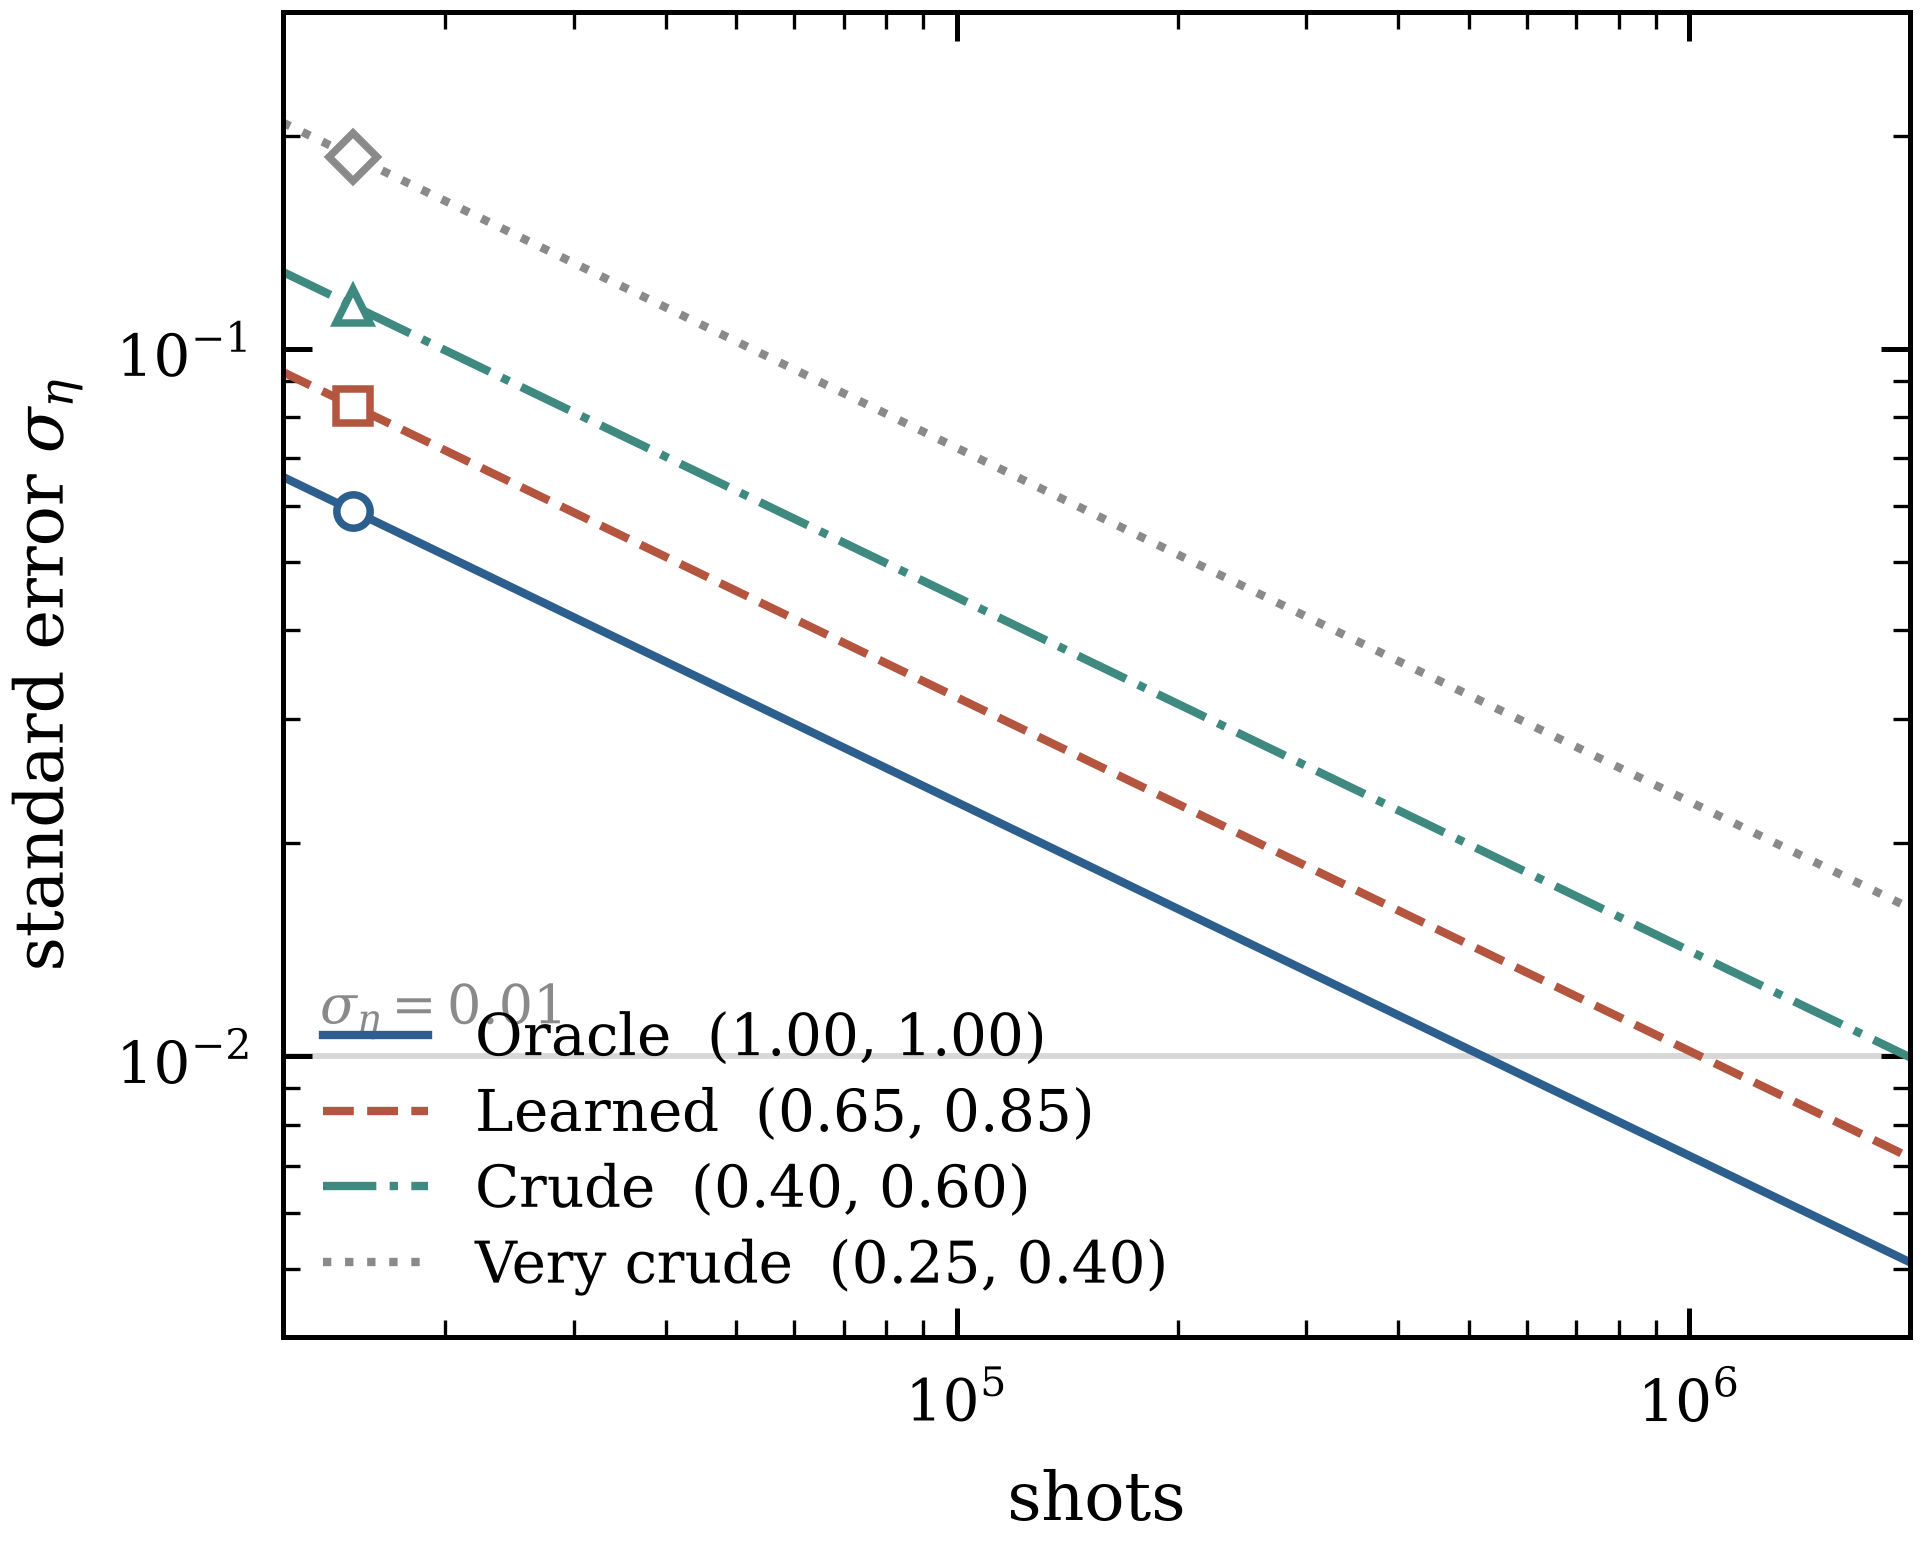
\includegraphics[width=\columnwidth]{figures/fig3_shotcost.png}
\caption{Estimator standard error versus shot count for four qualities of
upstream loss localization, written as (recall, precision). Markers are
measured at $1.5\times10^{4}$ shots; lines are the $1/\sqrt{N}$ projection.
A localizer wrong three times in four stays within about a factor of three of
an oracle.}
\label{fig:shotcost}
\end{figure}
\label{sec:res-localizer}

Equation~\eqref{eq:estimator} needs to know which ancilla to read, so something
upstream has to say when and where a loss happened. We degrade that step on
purpose. The simulated localizer returns qubit and round but not the gate
substep, so all candidate partners are averaged, and it makes both
false-positive and timing errors. False positives push $\hat\eta$ up: a
phantom loss looks like a suppressed partner. Timing errors push it down.

Fig.~\ref{fig:shotcost} is the resulting standard error, projected to larger
$N$ as $1/\sqrt{N}$. A localizer with the recall and precision of the learned
decoder in Ref.~\cite{wang2026aiqubitloss} reaches $\sigma_\eta=0.010$ at
$10^{6}$ shots. A poor localizer that is wrong three times in four still
reaches $0.023$, about three times worse than an oracle. Memory experiments
already collect $10^{6}$ shots or more, so the estimator does not need a
strong loss decoder to be usable.

\subsection{Robustness Under Refined Neutral-Atom Noise}
\label{sec:res-realism}

The anchors do not move under the extra physics of
Sec.~\ref{sec:methods-realism}. Table~\ref{tab:realism} adds, one at a time,
the maximally biased $Z$ error on the surviving partner, the residual Pauli
budget of the measured two-qubit gate, and a false-bright rate. The first
anchor shifts by at most $0.0011$. The second tracks $1-\epsilon$ exactly.

The survivor bias is easy to dismiss. That error hits the atom that remains
after a one-sided loss. The estimator reads the ancilla of the atom that left.
A $Z$ on a live data qubit cannot make a missing ancilla read bright.

End-to-end recovery is unchanged as well. At $\eta=0.5$ with high statistics
the refined model gives $\hat\eta=0.4979\pm 0.0125$ against
$0.4931\pm 0.0124$ for the plain model. Sweeping $\epsilon$ from $0$ to
$0.05$ leaves every point of the $\eta$ recovery inside its interval.

\begin{table}[!t]
\caption{Estimator anchors under cumulative additions of refined neutral-atom
physics. Theory values are $0.5$ and $1-\epsilon$.}
\label{tab:realism}
\centering
\begin{tabular}{@{}lcc@{}}
\toprule
Noise model & Partner alive & Partner co-lost \\
\midrule
Gate-cancellation loss only & 0.5006 & 1.0000 \\
$+$ survivor biased $Z$ & 0.5000 & 1.0000 \\
$+$ residual Pauli budget & 0.4999 & 1.0000 \\
$+$ false-bright $\epsilon=0.01$ & 0.4995 & 0.9900 \\
\bottomrule
\end{tabular}
\end{table}

\subsection{Generality Across Codes and Distances}
\label{sec:res-generality}

Section~\ref{sec:theory-detector} depends only on whether a stabilizer sign is
randomly projected. The experiments agree. Forcing a single ancilla dead at a
bulk round, the raw outcome is $0$ with probability $1.0000$ on every code and
distance tested. Its detector fires with probability $0$ on the deterministic
type and $0.5$ on the projected type.

The color code is the useful check because it flips the labels. In a
memory-$Z$ surface-code experiment the $Z$-type ancillas are deterministic
(steady-state mean $0.000$) and the $X$-type are projected ($0.499$). In the
color code the $Z$-type ancillas measure a projected stabilizer (mean
$0.498$), and their detectors are blind. Which type is blind depends on the
code and the basis. That the projected type is blind does not.

Table~\ref{tab:generality} runs the full pipeline across codes. The color code
has six layers per round, not four. The unrotated surface code keeps four
layers but changes the stabilizer geometry. In both cases the anchors hold
and $\eta$ is recovered inside confidence intervals over its full range.

\begin{table}[!t]
\caption{Estimator across code families. ``Layers'' is the number of two-qubit
gate layers per extraction round, read from the circuit. Data/ancilla counts are quoted at $d=5$.}
\label{tab:generality}
\centering
\begin{tabular}{@{}lccccc@{}}
\toprule
Code & $d$ & Data/anc & Layers & Alive & Co-lost \\
\midrule
Rotated surface & 3, 5, 7 & 25/24 & 4 & 0.5000 & 1.0000 \\
Unrotated surface & 5 & 41/40 & 4 & 0.5005 & 1.0000 \\
Color & 5 & 19/9 & \textbf{6} & 0.5009 & 1.0000 \\
\bottomrule
\end{tabular}
\end{table}

\subsection{Effect of Knowing $\eta$ on Decoding}
\begin{figure}[!t]
\centering
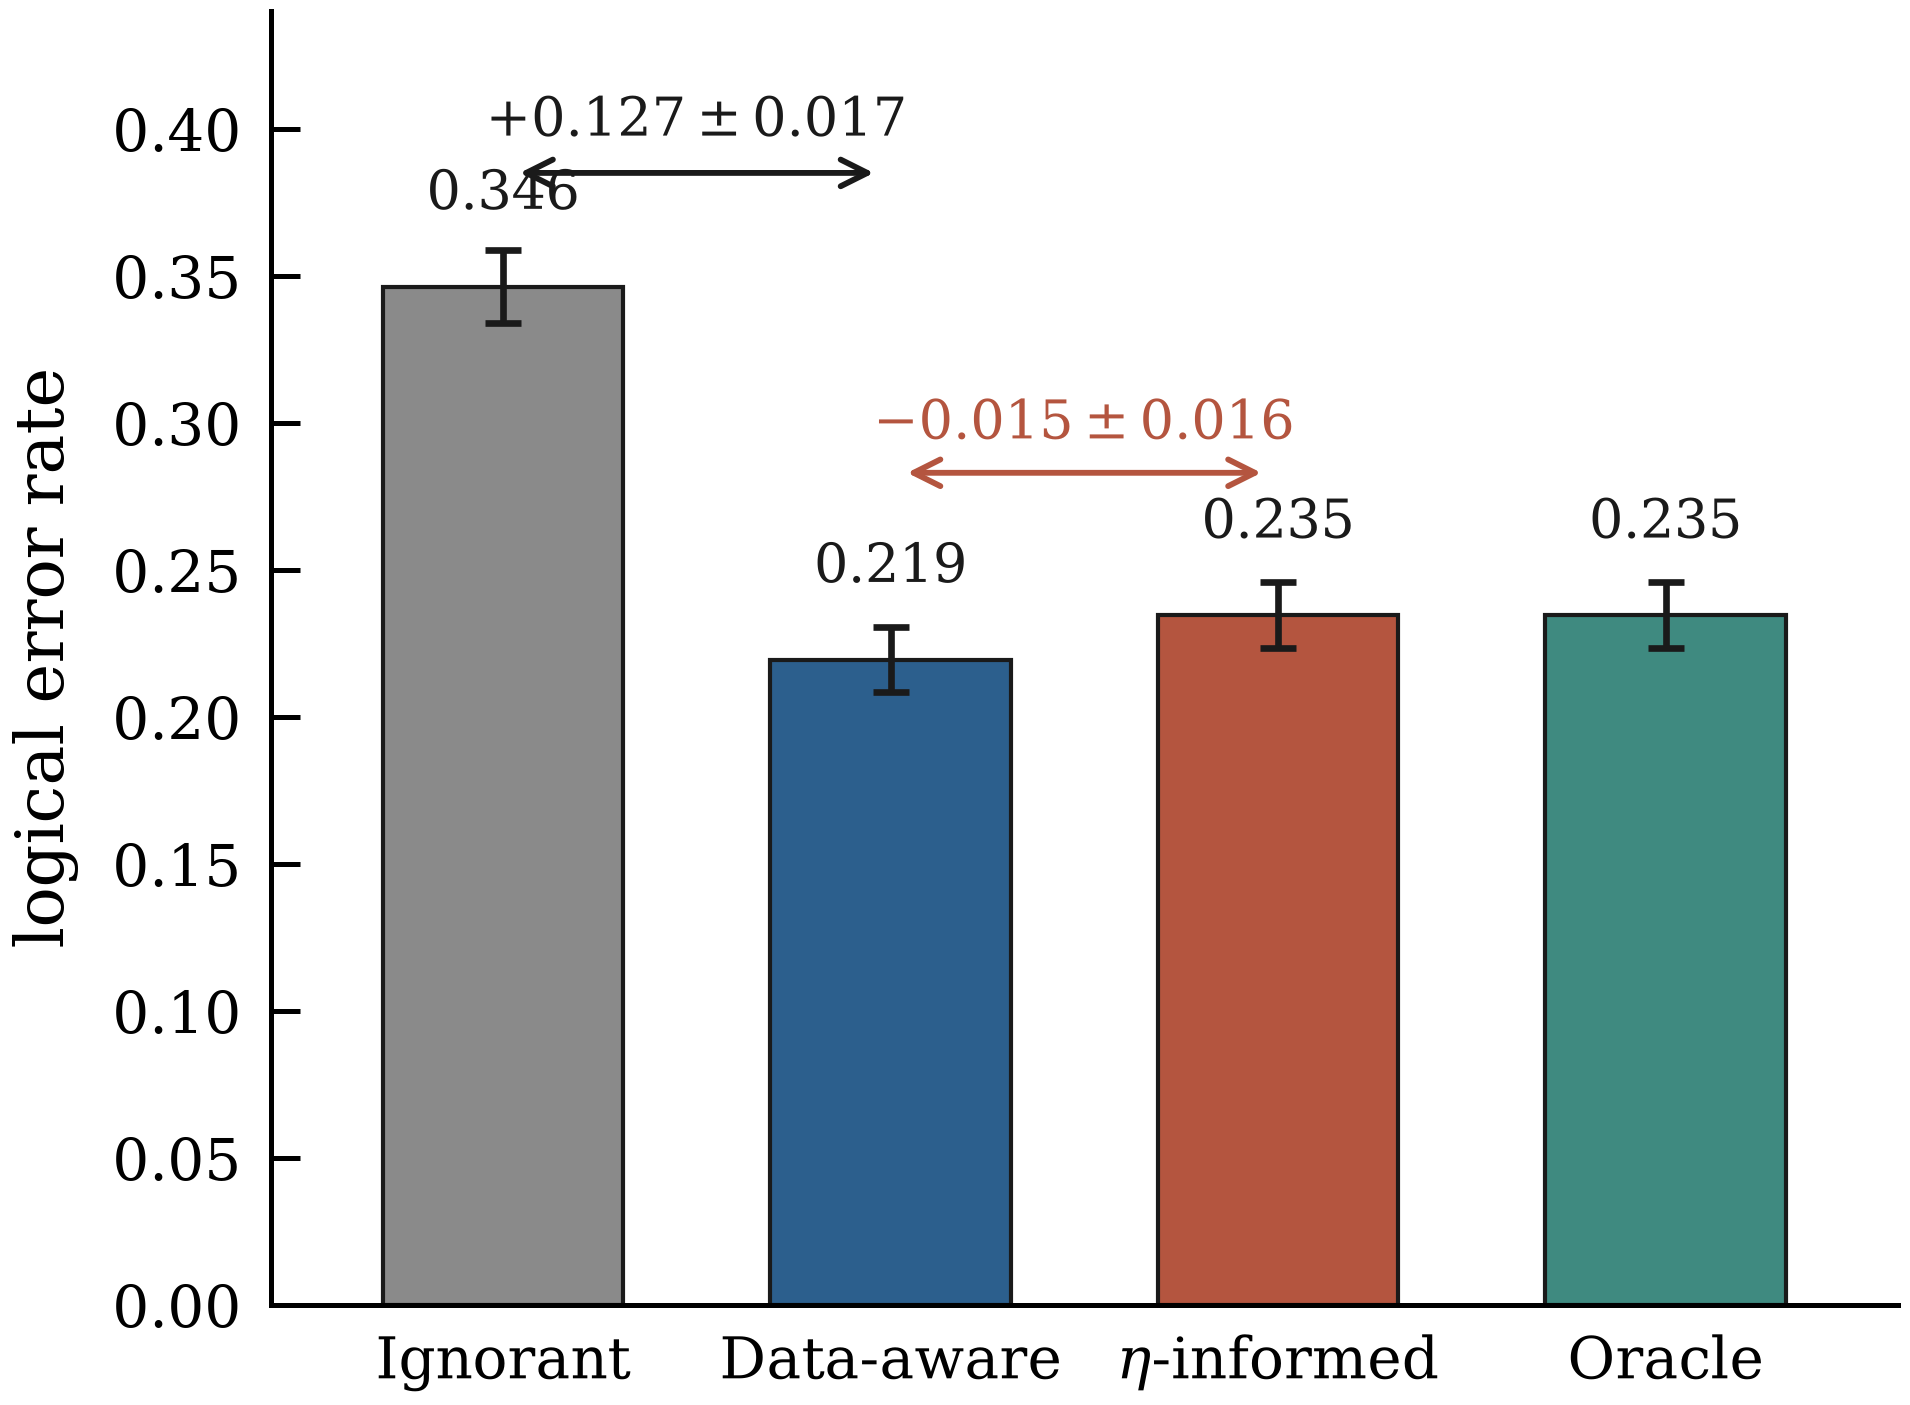
\includegraphics[width=\columnwidth]{figures/fig4_impact.png}
\caption{Logical error rate under four decoder belief models at
$p_g=8\times10^{-3}$, $\eta=1$, $5500$ shots. Error bars are $95\%$
confidence intervals. The gap between the ignorant and data-aware arms shows
that the decoder uses loss information when it has it, so the null between
the data-aware and $\eta$-informed arms is a real null. The oracle arm, given
every dead ancilla, sits on top of the $\eta$-informed arm.}
\label{fig:impact}
\end{figure}
\label{sec:res-impact}

A natural question is whether handing $\eta$ to a decoder lowers the logical
error rate. For the most direct strategy that does not use loss heralds, it
does not.

The same lossy syndrome data is decoded four ways. The arms differ only in
what the decoder is told about losses. A lossy circuit has non-deterministic
detectors and a non-deterministic logical observable, so we sample from the
true lossy circuit and decode against the clean detector error model, changing
edge weights per shot to encode the decoder's beliefs. Matching is
minimum-weight perfect matching~\cite{higgott2022pymatching,higgott2025sparseblossom}.
Freeing an edge means setting its probability to $1/2$. Rebuilding the model
with no modification reproduces the baseline logical error rate exactly.

Fig.~\ref{fig:impact} is the comparison. The control is not small. A decoder
told nothing about losses sits at $0.346$. The same decoder told the
data-qubit loss locations sits at $0.219$, a drop of $0.127\pm 0.017$. The
decoder uses loss information when it has it. A null among the remaining arms
is therefore a real null, not a dead instrument.

Also telling the decoder which ancillas were co-lost, so it can discount those
syndrome bits, does not help: $0.235$ against $0.219$, a difference of
$-0.015\pm 0.016$. The shift is consistently negative across runs and machines
but not significant on its own. That is not a problem with the quality of
$\hat\eta$. An oracle that is given every dead ancilla returns the same
logical error rate as the $\eta$-informed arm, because at $\eta=1$ the
informed belief is the truth.

The reason is the same as Sec.~\ref{sec:theory-anchors}. Discounting a
co-lost ancilla treats its reading as erased. A dead ancilla reads zero
every time---that is the fact the estimator uses---and its detector still
constrains the previous round. Erasing the bit throws away more than the
correction puts back.

This is one strategy, not a verdict on $\eta$ in every decoder.
Ref.~\cite{perrin2026correlatedloss} uses the same correlation inside a loss
graph built from teleportation-based heralds and reports up to an
order-of-magnitude drop in logical error probability, with a threshold move
from $3.2\%$ to $4\%$. That construction needs hardware this paper does not
assume. Putting an estimated $\eta$ into a herald-based decoder of that kind
is left open.


\section{Discussion}
\label{sec:discussion}

\subsection{What the Estimator Supplies}
\label{sec:disc-purpose}

The correlation parameter is already established in the neutral-atom
error-correction literature, and it already carries quantitative consequences.
Ref.~\cite{perrin2026correlatedloss} sweeps it from $0$ to $1$ and reports the
loss threshold moving from $3.2\%$ to $4\%$;
Ref.~\cite{liu2026optimaldistanceatomloss} sweeps the same quantity and reports
a threshold moving from $5.15\%$ to $7.82\%$. Both treat it as a free input,
because measuring it has required either loss-resolving readout or dedicated
loss-detection circuitry.

Equation~\eqref{eq:estimator} closes that measurement gap with data a standard
memory experiment already collects. Once $\eta$ can be reported alongside gate
fidelity and per-atom loss rate, a platform can tell which point on the
published threshold curves it actually occupies, and whether
correlated-loss-aware decoding is worth building for that hardware.

The benefit of correlated loss reported in those works does not make the
measurement unnecessary. The benefit is a curve, not a constant: $\eta=0.3$ and
$\eta=0.9$ imply different thresholds and resource estimates. Those studies
quantify the payoff; neither determines which payoff a given device receives.

\subsection{Relation to Syndrome-Statistics Estimation}
\label{sec:disc-relation}

Estimating error-model parameters from syndrome data is a standard
program~\cite{spitz2018adaptiveweight,blumekohout2025detectorerrormodels}. It
is built on the detector record, which is the right record for Pauli and
measurement errors. Sec.~\ref{sec:res-representation} shows that the same
record is blind to correlated atom loss on the randomly projected half of the
stabilizer group. Sec.~\ref{sec:theory-detector} says why: loss pins an
outcome to zero whether or not the gauge that the detector map quotients away
is present.

The two tools are for different error classes. Detector-based estimators stay
the right tool for the mechanisms they were written for. Atom loss needs a
different observable from the same experiment. Equation~\eqref{eq:estimator}
is one thing that observable makes available.

\subsection{Reconciling the Decoding Result}
\label{sec:disc-decoding}

Section~\ref{sec:res-impact} finds no decoding gain from supplying $\eta$.
Ref.~\cite{perrin2026correlatedloss} reports up to an order-of-magnitude drop
in logical error probability from using the same correlation. The difference
is how the number is used.

Their decoder takes heralds from teleportation-based detection units, which
say where atoms are missing, and uses the correlation to update loss
probabilities on a graph built from those heralds. The strategy tested here
has no heralds, by design: the premise is that the extra hardware is absent.
The only use of $\eta$ then available is to discount syndrome bits from
ancillas believed to be co-lost.

That use fails for a reason already in this paper. A dead ancilla reads zero
deterministically, which is \eqref{eq:anchor2}, and its detector still
constrains the previous round. Treating the bit as erased discards information.
The oracle arm makes the diagnosis sharp: perfect knowledge of every dead
ancilla matches the $\eta$-informed arm, so the null is about the strategy,
not about the estimate.

The claim is therefore narrow. Knowing $\eta$ does not help
detector-discounting decoding without heralds. Whether an estimated $\eta$
helps a herald-based decoder of the kind in
Ref.~\cite{perrin2026correlatedloss} is a different question and needs
superstabilizer machinery that is not implemented here.

\subsection{Limitations}
\label{sec:disc-limitations}

The experiments are memory experiments in one basis at a time. Logical
circuits with transversal gates, lattice surgery, or code deformation are not
tested, and the anchors in Sec.~\ref{sec:theory-anchors} are derived for the
memory setting.

The codes are CSS codes with a data--ancilla gate schedule and at most one
gate per qubit per layer. That covers the surface and color codes reported
here. It does not cover extraction circuits that break those assumptions.

The noise model is circuit-level depolarizing noise plus the refined loss
physics in Sec.~\ref{sec:methods-realism}. It does not include crosstalk,
transport or shuttling loss between rounds, or correlated non-Markovian
effects. No hardware record is used. The estimator has not been run on an
experimental syndrome file.

The refined-physics path is checked by the anchor tests and by end-to-end
agreement with the plain model. It is not checked byte-for-byte against the
audited reference builder, which does not implement those extra effects.

The decoding question in Sec.~\ref{sec:res-impact} is one strategy at one
operating point. The measured difference is consistently negative across
independent runs and is not significant on its own. We do not claim that
knowing $\eta$ hurts decoding. We claim that this strategy does not benefit
from it.

\subsection{Explicit Non-Claims}
\label{sec:disc-nonclaims}

Raw stabilizer outcomes are not claimed as a new representation. That choice
is already in the leakage literature
\cite{bultink2020repetitiveparity,varbanov2020leakagedetection} and in a
learned atom-loss decoder that consumes both raw bits and
detectors~\cite{wang2026aiqubitloss}. The contribution is the estimand and
the closed form: a calibration-free estimator of the gate-pair loss
correlation, a measured representation gap, and the argument that produces
the gap.

No advantage is claimed over herald-based correlated-loss decoders. Those
methods solve a different problem with additional hardware.

No experimental validation is claimed. Every result is simulation, checked
against known answers, not against a measured device record.

\subsection{Future Work}
\label{sec:disc-future}

Three next steps are immediate. The first is to run the estimator on an
experimental syndrome record from a neutral-atom device. That needs no new
theory and would turn the method into a measurement. The second is to put an
estimated $\eta$ into a herald-based decoder with superstabilizers, which is
the natural test of whether the parameter helps when it is used the way
Ref.~\cite{perrin2026correlatedloss} uses it. The third is to recover the
gate substep of a loss instead of averaging candidate partners. The substep
sits in the mixture of partner outcomes; using it would tighten $\sigma_\eta$
by about a factor of four at fixed shot count.


\section{Conclusion}
\label{sec:conclusion}

Correlated atom loss is a hardware property with published consequences for
error-correction performance, and until now it has been a parameter that
studies vary rather than measure. We have shown that it can be recovered in
closed form from the measurement record a surface-code memory experiment
already produces. The two constants in the formula are fixed by the code
structure and the readout mechanism rather than by calibration, and the
procedure does not require loss-resolving readout, extra detection circuitry,
or a trained model.

The estimator recovers the correlation within confidence intervals across its
full range, on three code families and three code distances, under a noise
model that includes biased errors on surviving atoms and a measured gate error
budget. It reaches a standard error of $0.010$ at $10^{6}$ shots when paired
with a loss localizer of currently published quality, and $0.023$ with a
deliberately poor one, so it does not depend on a strong loss decoder to be
useful.

We also report that supplying the correlation to a decoder that discounts
syndrome bits from co-lost ancillas does not reduce the logical error rate.
The reason is the same physics the estimator relies on: a dead ancilla's
reading is deterministic and therefore informative, so treating it as erased
discards more than it recovers. Whether the parameter improves decoding when
used inside a herald-based loss graph remains open.

The immediate application is characterization. A neutral-atom device can now
report its gate-pair loss correlation alongside its gate fidelity, and thereby
determine which point on the published threshold curves it occupies.



\section*{Acknowledgment}
The author thanks the developers of Stim and PyMatching, whose open-source
tools made the numerical work in this paper possible. The simulation code, the
complete suite of known-answer validation checks, and the scripts that generate
the figures are available at \url{https://github.com/Suriya-002/decoder}.
The author used Claude (Anthropic) to assist with language editing of the
manuscript after the technical content had been written. The assistance was
limited to grammar, wording, and readability. The problem statement,
derivations, experiments, figures, and conclusions are the author's.

\bibliographystyle{IEEEtran}
\bibliography{references}

\EOD

\end{document}